\documentclass[12pt]{report}
\usepackage{scribe,graphicx,graphics}
\usepackage{subcaption}


\course{MIT 22.213} 	
\coursetitle{Nuclear Reactor Kinetics}	
\semester{Spring 2015}
\lecturenumber{5}	
\lecturedate{}		


% Insert your name here!
\scribe{Geoffrey Gunow}

\begin{document}
	
	
	\maketitle
	
	\paragraph{Intro: Code Design}
	In this problem set, I extend the \texttt{rksolver} library to include a frequency transformed transient solver. This library is written in C++ for speed and includes a SWIG wrapper for Python. This allows for easy data entry and manipulation in Python while still being able to take advantage of the speed of C++.
	
	\paragraph{Derivation of Frequency Transform Equations}
	First, the frequency transform equations are derived which form the basis of the updates to \texttt{rksolver}. Starting from the multi-group group diffusion equation,
	\begin{eqnarray}
	\frac{\partial}{\partial t} \left\langle \frac{1}{v_g(\vec{r},t)} \phi_g(\vec{r},t) \right\rangle = \nabla D_g(\vec{r},t) \nabla \phi_g(\vec{r},t) - \Sigma_{t,g}(\vec{r},t) \phi_g(\vec{r},t) + \sum_{g'=1}^{G} \Sigma_{s}^{g'\rightarrow g} (\vec{r},t) \phi_{g'}(\vec{r},t) \nonumber \\ 
	+ \left[ 1- \beta(\vec{r},t) \right] \frac{\chi_g^p}{k_{crit}} \sum_{g'=1}^{G} \nu \Sigma_{f,g'}(\vec{r},t) \phi_{g'}(\vec{r},t) + \sum_{i=1}^{I} \chi_{i,g}^d \lambda_i C_i(\vec{r},t) \nonumber
	\end{eqnarray}
	note that
	\begin{equation}
	\Sigma_{t,g} = \Sigma_{a,g} + \sum_{g'= 1}^G \Sigma_{s}^{g\rightarrow g'} \nonumber.
	\end{equation}
	If $v_g$ and $\beta$ are assumed to be constant in both space and time, the balance equation reduces to
	\begin{eqnarray}
	\frac{\partial}{\partial t} \left( \frac{1}{v_g} \phi_g(\vec{r},t) \right) = \nabla D_g(\vec{r}) \nabla \phi_g(\vec{r},t)  - \Sigma_{a,g}(\vec{r},t) \phi_g(\vec{r},t) - \sum_{g'\neq g} \Sigma_{s}^{g\rightarrow g'} (\vec{r},t) \phi_{g}(\vec{r},t)  \nonumber \\  + \sum_{g' \neq g} \Sigma_{s}^{g'\rightarrow g} (\vec{r},t) \phi_{g'}(\vec{r},t)
	+ \left[ 1- \beta \right] \frac{\chi_g^p}{k_{crit}} \sum_{g'=1}^{G} \nu \Sigma_{f,g'}(\vec{r},t) \phi_{g'}(\vec{r},t) + \sum_{i=1}^{I} \chi_{i,g}^d \lambda_i C_i(\vec{r},t) \nonumber.
	\end{eqnarray}
	Now let $\phi_g(\vec{r},t) = \psi_g(\vec{r},t) e^{\omega_g(\vec{r}) (t-t_n)}$ which leads to
	\begin{eqnarray}
	\frac{\partial}{\partial t} \left( \frac{1}{v_g} \psi_g(\vec{r},t) e^{\omega_g(\vec{r}) (t-t_n)} \right) = \nabla D_g(\vec{r}) \nabla \psi_g(\vec{r},t) e^{\omega_g(\vec{r}) (t-t_n)}  - \Sigma_{a,g}(\vec{r},t) \psi_g(\vec{r},t) e^{\omega_g(\vec{r}) (t-t_n)} - \nonumber \\ \sum_{g'\neq g} \Sigma_{s}^{g\rightarrow g'} (\vec{r},t) \psi_g(\vec{r},t) e^{\omega_g(\vec{r}) (t-t_n)}    + \sum_{g' \neq g} \Sigma_{s}^{g'\rightarrow g} (\vec{r},t) \psi_{g'}(\vec{r},t) e^{\omega_{g'}(\vec{r}) (t-t_n)} \nonumber \\
	+ \left[ 1- \beta \right] \frac{\chi_g^p}{k_{crit}} \sum_{g'=1}^{G} \nu \Sigma_{f,g'}(\vec{r},t) \psi_{g'}(\vec{r},t) e^{\omega_{g'}(\vec{r}) (t-t_n)} + \sum_{i=1}^{I} \chi_{i,g}^d \lambda_i C_i(\vec{r},t) \nonumber
	\end{eqnarray}
	which can be expanded and simplified to
	\begin{eqnarray}
	\frac{1}{v_g} \frac{\partial \psi_g(\vec{r},t)}{\partial t} + \frac{\omega_g(\vec{r})}{v_g} \psi_g(\vec{r},t)  = \nabla D_g(\vec{r},t) \nabla \psi_g(\vec{r},t) - \Sigma_{a,g}(\vec{r},t) \psi_g(\vec{r},t) -  \sum_{g'\neq g} \Sigma_{s}^{g\rightarrow g'} (\vec{r},t) \psi_g(\vec{r},t) \nonumber \\ + e^{-\omega_g(\vec{r}) (t-t_n)} \sum_{g' \neq g} \Sigma_{s}^{g'\rightarrow g} (\vec{r},t) \psi_{g'}(\vec{r},t) e^{\omega_{g'}(\vec{r}) (t-t_n)} \nonumber \\
	+ \left[ 1- \beta \right] \frac{\chi_g^p}{k_{crit}} e^{-\omega_g(\vec{r}) (t-t_n)} \sum_{g'=1}^{G} \nu \Sigma_{f,g'}(\vec{r},t) \psi_{g'}(\vec{r},t) e^{\omega_{g'}(\vec{r}) (t-t_n)} \nonumber \\ + e^{-\omega_g(\vec{r}) (t-t_n)} \sum_{i=1}^{I} \chi_{i,g}^d \lambda_i C_i(\vec{r},t) \nonumber.
	\end{eqnarray}
	Turning to the precursors, the time rate of change for the precursors $C_i(\vec{r},t)$ can be expressed as
	\begin{equation}
	\frac{\partial}{\partial t} C_i(\vec{r},t) = -\lambda_i C_i(\vec{r},t) + \frac{\beta_i(\vec{r},t)}{k_{crit}} \sum_{g'=1}^{G} \nu \Sigma_{f,g'}(\vec{r},t) \phi_{g'}(\vec{r},t) \nonumber
	\end{equation}
	which can be rewritten as
	\begin{equation}
	\frac{\partial}{\partial t} C_i(\vec{r},t) = -\lambda_i C_i(\vec{r},t) + \frac{\beta_i(\vec{r},t)}{k_{crit}} \sum_{g'=1}^{G} \nu \Sigma_{f,g'}(\vec{r},t) \psi_{g'}(\vec{r},t) e^{\omega_{g'}(\vec{r}) (t-t_n)} \nonumber
	\end{equation}
	under the assumption that $\phi_g(\vec{r},t) = \psi_g(\vec{r},t) e^{\omega_g(\vec{r}) (t-t_n)}$. This can be re-written as
	\begin{eqnarray}
	\frac{\partial}{\partial t} \left( C_i(\vec{r},t) e^{\lambda_i t} \right) = \frac{\beta_i(\vec{r},t) e^{\lambda_i t}}{k_{crit}} \sum_{g'=1}^{G} \nu \Sigma_{f,g'}(\vec{r},t) \psi_{g'}(\vec{r},t) e^{\omega_{g'}(\vec{r}) (t-t_n)} \nonumber \\
	\int_{t=t_n}^{t=t_{n+1}} \partial \left( C_i(\vec{r},t) e^{\lambda_i t} \right) = \int_{t=t_n}^{t=t_{n+1}}  \partial t \, \frac{\beta_i(\vec{r},t) e^{\lambda_i t}}{k_{crit}} \sum_{g'=1}^{G} \nu \Sigma_{f,g'}(\vec{r},t) \psi_{g'}(\vec{r},t) e^{\omega_{g'}(\vec{r}) (t-t_n)} \nonumber \\
	 C_i(\vec{r},t_{n+1}) e^{\lambda_i t_{n+1}} - C_i(\vec{r},t_{n}) e^{\lambda_i t_{n}} = \int_{t=t_n}^{t=t_{n+1}}  \partial t \, \frac{\beta_i(\vec{r},t) e^{\lambda_i t}}{k_{crit}} \sum_{g'=1}^{G} \nu \Sigma_{f,g'}(\vec{r},t) \psi_{g'}(\vec{r},t) e^{\omega_{g'}(\vec{r}) (t-t_n)} \nonumber \\
	 C_i(\vec{r},t_{n+1}) =  C_i(\vec{r},t_{n}) e^{-\lambda_i \Delta t} +  \int_{t=t_n}^{t=t_{n+1}}  \partial t \, \frac{\beta_i(\vec{r},t) e^{-\lambda_i \left(t_{n+1} - t \right)}}{k_{crit}} \sum_{g'=1}^{G} \nu \Sigma_{f,g'}(\vec{r},t) \psi_{g'}(\vec{r},t) e^{\omega_{g'}(\vec{r}) (t-t_n)} \nonumber
	\end{eqnarray}	
	where $\Delta t = t_{n+1} - t_n$. Assuming $\nu \Sigma_{f,g'}(\vec{r},t)$ is constant over the interval $(t_n, t_{n+1})$ and the flux factor $\psi_{g'}(\vec{r},t)$ varies linearly with time as
	\begin{equation}
	\psi_{g'}(\vec{r},t) = \psi_{g'}(\vec{r},t_n) \frac{t_{n+1}-t}{\Delta t} + \psi_{g'}(\vec{r},t_{n+1}) \frac{t-t_n}{\Delta t} 
	\end{equation}
	the precursor equation transforms to
	\begin{eqnarray}
	C_i(\vec{r},t_{n+1}) =  C_i(\vec{r},t_{n}) e^{-\lambda_i \Delta t} + \nonumber \\  \int_{t=t_n}^{t=t_{n+1}}  \partial t \, \frac{\beta_i(\vec{r},t) e^{-\lambda_i \left(t_{n+1} - t \right)}}{k_{crit}} \sum_{g'=1}^{G} \nu \Sigma_{f,g'}(\vec{r},t_{n+1}) \left( \psi_{g'}(\vec{r},t_n) \frac{t_{n+1}-t}{\Delta t} \ + \psi_{g'}(\vec{r},t_{n+1}) \frac{t-t_n}{\Delta t} \right) e^{\omega_{g'}(\vec{r}) (t-t_n)}. \nonumber
	\end{eqnarray}
	Assuming that $\beta(\vec{r},t)$ is constant over space and time,
	\begin{eqnarray}
	C_i(\vec{r},t_{n+1}) =  C_i(\vec{r},t_{n}) e^{-\lambda_i \Delta t} + \nonumber \\  \sum_{g'=1}^{G} e^{-\left(\lambda_i t_{n+1} + \omega_{g'}(\vec{r})t_n \right)} \int_{t=t_n}^{t=t_{n+1}}  \partial t \, \frac{\beta_i e^{\left(\lambda_i + \omega_{g'}(\vec{r}) \right)  t}}{k_{crit}}  \nu \Sigma_{f,g'}(\vec{r},t_{n+1}) \left( \psi_{g'}(\vec{r},t_n) \frac{t_{n+1}-t}{\Delta t} + \psi_{g'}(\vec{r},t_{n+1}) \frac{t-t_n}{\Delta t}  \right). \nonumber
	\end{eqnarray}
	After some re-arranging, this expression can be re-written as two separate integrals
	\begin{eqnarray}
	C_i(\vec{r},t_{n+1}) =  C_i(\vec{r},t_{n}) e^{-\lambda_i \Delta t} + \nonumber \\  \sum_{g'=1}^{G} \frac{\beta_i \nu\Sigma_f(\vec{r},t_{n+1})}{k_{crit} \Delta t} e^{-\left(\lambda_i t_{n+1} + \omega_{g'}(\vec{r}) t_n \right)} 
	\times \nonumber \\ 
	\left(  \Delta(\psi_{g'}) \int_{t=t_n}^{t=t_{n+1}}  \partial t \, t e^{\left(\lambda_i + \omega_{g'}(\vec{r}) \right)  t} - \Delta(\psi_{g'} t) \int_{t=t_n}^{t=t_{n+1}}  \partial t \, e^{\left(\lambda_i + \omega_{g'}(\vec{r}) \right)  t} \right) \nonumber
	\end{eqnarray}
	where $\Delta(\psi_{g'}) =   \psi_{g'}(\vec{r},t_{n+1}) - \psi_{g'}(\vec{r},t_n)$ and $\Delta(\psi_{g'}t) =   \psi_{g'}(\vec{r},t_{n+1}) t_n - \psi_{g'}(\vec{r},t_n) t_{n+1}$. Solving these integrals,	
	\begin{eqnarray}
	C_i(\vec{r},t_{n+1}) =  C_i(\vec{r},t_{n}) e^{-\lambda_i \Delta t} + \nonumber \\  \sum_{g'=1}^{G} \frac{\beta_i \nu\Sigma_f(\vec{r},t_{n+1}) \Delta(\psi_{g'})}{k_{crit} \Delta t} e^{-\left(\lambda_i t_{n+1} + \omega_{g'}(\vec{r}) t_n \right)}  \left( \frac{t_{n+1} e^{\left(\lambda_i + \omega_{g'}(\vec{r}) \right)  t_{n+1}} - t_n e^{\left(\lambda_i + \omega_{g'}(\vec{r}) \right)  t_{n}}}{\lambda_i + \omega_{g'}(\vec{r})} \right) \nonumber \\
	- \sum_{g'=1}^{G} \frac{\beta_i\nu\Sigma_f(\vec{r},t_{n+1}) \Delta(\psi_{g'})}{k_{crit} \Delta t} e^{-\left(\lambda_i t_{n+1} + \omega_{g'}(\vec{r}) t_n \right)} \left( \frac{e^{\left(\lambda_i + \omega_{g'}(\vec{r}) \right)  t_{n+1}} - e^{\left(\lambda_i + \omega_{g'}(\vec{r}) \right)  t_{n}}}{\left(\lambda_i + \omega_{g'}(\vec{r})\right)^2}\right)
	 \nonumber \\ 
	 - \sum_{g'=1}^{G} \frac{\beta_i\nu\Sigma_f(\vec{r},t_{n+1}) \Delta(\psi_{g'}t)}{k_{crit} \Delta t} e^{-\left(\lambda_i t_{n+1} + \omega_{g'}(\vec{r}) t_n \right)} \left(\frac{e^{\left(\lambda_i + \omega_{g'}(\vec{r}) \right)  t_{n+1}} - e^{\left(\lambda_i + \omega_{g'}(\vec{r}) \right)  t_{n}}}{\lambda_i + \omega_{g'}(\vec{r})}\right) \nonumber
	\end{eqnarray}
	which can be simplified to
	\begin{eqnarray}
	C_i(\vec{r},t_{n+1}) =  C_i(\vec{r},t_{n}) e^{-\lambda_i \Delta t} + \nonumber \\  \sum_{g'=1}^{G} \frac{\beta_i \nu\Sigma_f(\vec{r},t_{n+1})}{k_{crit} \Delta t \left(\lambda_i + \omega_{g'}(\vec{r})\right)} e^{ \omega_{g'}(\vec{r}) \Delta t} \left( t_{n+1} \Delta(\psi_{g'}) - \Delta(\psi_{g'}t) - \frac{\Delta(\psi_{g'})}{\lambda_i + \omega_{g'}(\vec{r})} \right) \nonumber \\ 
	- \sum_{g'=1}^{G} \frac{\beta_i \nu\Sigma_f(\vec{r},t_{n+1})}{k_{crit} \Delta t \left(\lambda_i + \omega_{g'}(\vec{r})\right)} e^{-\lambda_i \Delta t} \left( t_{n} \Delta(\psi_{g'}) - \Delta(\psi_{g'}t) - \frac{\Delta(\psi_{g'})}{\lambda_i + \omega_{g'}(\vec{r})} \right). \nonumber
	\end{eqnarray}	
	Reinserting the definitions of $\Delta(\psi_{g'})$ and $\Delta(\psi_{g'}t)$,
	\begin{eqnarray}
	C_i(\vec{r},t_{n+1}) =  C_i(\vec{r},t_{n}) e^{-\lambda_i \Delta t} + \nonumber \\  \sum_{g'=1}^{G} \frac{\beta_i \nu\Sigma_f(\vec{r},t_{n+1})}{k_{crit} \Delta t \left(\lambda_i + \omega_{g'}(\vec{r})\right)} e^{ \omega_{g'}(\vec{r}) \Delta t} \left( \psi_{g'}(t_{n+1}) \Delta t - \frac{\psi_{g'}(t_{n+1})-\psi_{g'}(t_{n})}{\lambda_i + \omega_{g'}(\vec{r})} \right) \nonumber \\ 
	- \sum_{g'=1}^{G} \frac{\beta_i \nu\Sigma_f(\vec{r},t_{n+1})}{k_{crit} \Delta t \left(\lambda_i + \omega_{g'}(\vec{r})\right)} e^{-\lambda_i \Delta t} \left( \psi_{g'}(t_{n}) \Delta t - \frac{\psi_{g'}(t_{n+1})-\psi_{g'}(t_{n})}{\lambda_i + \omega_{g'}(\vec{r})} \right) \nonumber.
	\end{eqnarray}
	Defining factors
	\begin{equation}
	A_{g'} = \frac{\beta_i \nu\Sigma_f(\vec{r},t_{n+1})}{k_{crit} \Delta t \left(\lambda_i + \omega_{g'}(\vec{r})\right)}
	\end{equation}
	and
	\begin{equation}
	B_{g'} = \frac{\psi_{g'}(t_{n+1})-\psi_{g'}(t_{n})}{\lambda_i + \omega_{g'}(\vec{r})}
	\end{equation}
	leads to a condensed form of the precursor equations as
	\begin{eqnarray}
	C_i(\vec{r},t_{n+1}) =  C_i(\vec{r},t_{n}) e^{-\lambda_i \Delta t} +  \sum_{g'=1}^{G} A_{g'} \left( \left( \psi_{g'}(t_{n+1}) \Delta t - B_{g'} \right) e^{ \omega_{g'}(\vec{r}) \Delta t} - 
	\left( \psi_{g'}(t_n) \Delta t - B_{g'} \right) e^{-\lambda_i \Delta t} \right) \nonumber.
	\end{eqnarray}
	However a more useful form is
	\begin{eqnarray}
	C_i(\vec{r},t_{n+1}) =  C_i(\vec{r},t_{n}) e^{-\lambda_i \Delta t} \nonumber \\ 
	+ \sum_{g'=1}^{G} A_{g'} \psi_{g'}(t_{n+1}) \left( \left( \Delta t - \frac{1}{\lambda_i + \omega_{g'}(\vec{r})} \right) e^{\omega_{g'}(\vec{r}) \Delta t} + \frac{e^{-\lambda_i \Delta t}}{\lambda_i + \omega_{g'}(\vec{r})} \right) \nonumber \\
	- \sum_{g'=1}^{G} A_{g'} \psi_{g'}(t_{n}) \left( \frac{-e^{\omega_{g'}(\vec{r}) \Delta t}}{\lambda_i + \omega_{g'}(\vec{r})} + \left(\Delta t + \frac{1}{\lambda_i + \omega_{g'}(\vec{r})} \right)e^{-\lambda_i \Delta t} \right) \nonumber
	\end{eqnarray}
	as the contributions from $\psi_{g'}(t_{n+1})$ and $\psi_{g'}(t_{n})$ are separated. Returning to the neutron balance equation, the fully implicit finite difference approximation can be applied as
	\begin{eqnarray}
		 \frac{1}{v_g} \left(\frac{\psi_g(\vec{r},t_{n+1}) - \psi_g(\vec{r},t_{n})}{\Delta t} \right) + \frac{\omega_g(\vec{r})}{v_g} \psi_g(\vec{r},t_{n+1})  = \nabla D_g(\vec{r}) \nabla \psi_g(\vec{r},t_{n+1}) \nonumber \\ - \Sigma_{a,g}(\vec{r},t_{n+1}) \psi_g(\vec{r},t_{n+1}) - \sum_{g'\neq g} \Sigma_{s}^{g\rightarrow g'} (\vec{r},t_{n+1}) \psi_g(\vec{r},t_{n+1}) \nonumber \\ + e^{-\omega_g(\vec{r}) \Delta t} \sum_{g' \neq g} \Sigma_{s}^{g'\rightarrow g} (\vec{r},t_{n+1}) \psi_{g'}(\vec{r},t_{n+1}) e^{\omega_{g'}(\vec{r}) \Delta t} \nonumber \\
		+ \left[ 1- \beta \right] \frac{\chi_g^p}{k_{crit}} e^{-\omega_g(\vec{r}) \Delta t} \sum_{g'=1}^{G} \nu \Sigma_{f,g'}(\vec{r},t_{n+1}) \psi_{g'}(\vec{r},t_{n+1}) e^{\omega_{g'}(\vec{r}) \Delta t} \nonumber \\ + e^{-\omega_g(\vec{r}) \Delta t} \sum_{i=1}^{I} \chi_{i,g}^d \lambda_i C_i(\vec{r},t_{n+1}) \nonumber.
	\end{eqnarray}
	Inserting the definition for $C_i(\vec{r},t_{n+1})$ into the balance equation,
	\begin{eqnarray}
	\left(\frac{\psi_g(\vec{r},t_{n+1}) - \psi_g(\vec{r},t_{n})}{\Delta t} \right) \frac{\omega_g(\vec{r})}{v_g}  = \nabla D_g(\vec{r}) \nabla \psi_g(\vec{r},t_{n+1}) - \Sigma_{a,g}(\vec{r},t_{n+1}) \psi_g(\vec{r},t_{n+1}) -  \nonumber \\ \sum_{g'\neq g} \Sigma_{s}^{g\rightarrow g'} (\vec{r},t_{n+1}) \psi_g(\vec{r},t_{n+1}) + e^{-\omega_g(\vec{r}) \Delta t} \sum_{g' \neq g} \Sigma_{s}^{g'\rightarrow g} (\vec{r},t_{n+1}) \psi_{g'}(\vec{r},t_{n+1}) e^{\omega_{g'}(\vec{r}) \Delta t} \nonumber \\
	+ \left[ 1- \beta \right] \frac{\chi_g^p}{k_{crit}} e^{-\omega_g(\vec{r}) \Delta t} \sum_{g'=1}^{G} \nu \Sigma_{f,g'}(\vec{r},t_{n+1}) \psi_{g'}(\vec{r},t_{n+1}) e^{\omega_{g'}(\vec{r}) \Delta t} \nonumber \\ +  \sum_{i=1}^{I} \chi_{i,g}^d \lambda_i C_i(\vec{r},t_{n}) e^{-\left(\lambda_i + \omega_g(\vec{r})\right) \Delta t} \nonumber \\
	- \sum_{i=1}^{I} \chi_{i,g}^d \lambda_i \sum_{g'=1}^{G} A_{g'} \psi_{g'}(t_n) \left( \frac{-1}{\lambda_i + \omega_{g'}(\vec{r})} + \left(\Delta t + \frac{1}{\lambda_i + \omega_{g'}(\vec{r})} \right)e^{-\left(\lambda_i + \omega_{g'}(\vec{r}) \right) \Delta t} \right) \nonumber \\
	+ \sum_{i=1}^{I} \chi_{i,g}^d \lambda_i \sum_{g'=1}^{G} A_{g'} \psi_{g'}(t_{n+1}) \left( \Delta t - \frac{1}{\lambda_i + \omega_{g'}(\vec{r})} + \frac{e^{-\left( \lambda_i + \omega_{g'}(\vec{r}) \right) \Delta t}}{\lambda_i + \omega_{g'}(\vec{r})} \right)
	\nonumber
	\end{eqnarray}
	which can be simplified as
	\begin{eqnarray}
	\frac{1}{v_g} \left(\frac{\psi_g(\vec{r},t_{n+1}) - \psi_g(\vec{r},t_{n})}{\Delta t} \right) + \frac{\omega_g(\vec{r})}{v_g} \psi_g(\vec{r},t_{n+1})  = \nabla D_g(\vec{r}) \nabla \psi_g(\vec{r},t_{n+1}) - \Sigma_{a,g}(\vec{r},t_{n+1}) \psi_g(\vec{r},t_{n+1}) -  \nonumber \\ \sum_{g'\neq g} \Sigma_{s}^{g\rightarrow g'} (\vec{r},t_{n+1}) \psi_g(\vec{r},t_{n+1}) + \sum_{g' \neq g} \Sigma_{s}^{g'\rightarrow g} (\vec{r},t_{n+1}) \psi_{g'}(\vec{r},t_{n+1}) e^{\left(\omega_{g'}(\vec{r}) - \omega_{g}(\vec{r}) \right) \Delta t} \nonumber \\
	+ \left[ 1- \beta \right] \frac{\chi_g^p}{k_{crit}} \sum_{g'=1}^{G} \nu \Sigma_{f,g'}(\vec{r},t_{n+1}) \psi_{g'}(\vec{r},t_{n+1}) e^{\left(\omega_{g'}(\vec{r}) - \omega_{g}(\vec{r}) \right) \Delta t} \nonumber \\ +  \sum_{i=1}^{I} \chi_{i,g}^d \lambda_i C_i(\vec{r},t_{n}) e^{-\left(\lambda_i + \omega_g(\vec{r})\right) \Delta t} \nonumber \\
	- \sum_{i=1}^{I} chi_{i,g}^d \lambda_i \sum_{g'=1}^{G} A_{g'} \psi_{g'}(t_n) \left( \frac{-1}{\lambda_i + \omega_{g'}(\vec{r})} + \left(\Delta t + \frac{1}{\lambda_i + \omega_{g'}(\vec{r})} \right)e^{-\left(\lambda_i + \omega_{g'}(\vec{r}) \right) \Delta t} \right) \nonumber \\
	+ \sum_{i=1}^{I} \chi_{i,g}^d \lambda_i \sum_{g'=1}^{G} A_{g'} \psi_{g'}(t_{n+1}) \left( \Delta t - \frac{1}{\lambda_i + \omega_{g'}(\vec{r})} + \frac{e^{-\left( \lambda_i + \omega_{g'}(\vec{r}) \right) \Delta t}}{\lambda_i + \omega_{g'}(\vec{r})} \right)
	\nonumber.
	\end{eqnarray}
	Assuming $\omega_{g'}(\vec{r}) = \omega_g(\vec{r}) = \omega(\vec{r})$,
	\begin{eqnarray}
	\frac{1}{v_g} \left(\frac{\psi_g(\vec{r},t_{n+1}) - \psi_g(\vec{r},t_{n})}{\Delta t} \right) + \frac{\omega(\vec{r})}{v_g} \psi_g(\vec{r},t_{n+1})  = \nabla D_g(\vec{r}) \nabla \psi_g(\vec{r},t_{n+1}) \nonumber \\ - \Sigma_{a,g}(\vec{r},t_{n+1}) \psi_g(\vec{r},t_{n+1}) -   \sum_{g'\neq g} \Sigma_{s}^{g\rightarrow g'} (\vec{r},t_{n+1}) \psi_g(\vec{r},t_{n+1}) + \sum_{g' \neq g} \Sigma_{s}^{g'\rightarrow g} (\vec{r},t_{n+1}) \psi_{g'}(\vec{r},t_{n+1}) \nonumber \\
	+ \left[ 1- \beta \right] \frac{\chi_g^p}{k_{crit}} \sum_{g'=1}^{G} \nu \Sigma_{f,g'}(\vec{r},t_{n+1}) \psi_{g'}(\vec{r},t_{n+1})  +  \sum_{i=1}^{I} \chi_{i,g}^d \lambda_i C_i(\vec{r},t_{n}) e^{-\left(\lambda_i + \omega(\vec{r})\right) \Delta t} \nonumber \\
	- \sum_{i=1}^{I} \chi_{i,g}^d \lambda_i \sum_{g'=1}^{G} A_{g'} \psi_{g'}(t_n) \left( \frac{-1}{\lambda_i + \omega(\vec{r})} + \left(\Delta t + \frac{1}{\lambda_i + \omega(\vec{r})} \right)e^{-\left(\lambda_i + \omega(\vec{r}) \right) \Delta t} \right) \nonumber \\
	+ \sum_{i=1}^{I} \chi_{i,g}^d \lambda_i \sum_{g'=1}^{G} A_{g'} \psi_{g'}(t_{n+1}) \left( \Delta t - \frac{1}{\lambda_i + \omega(\vec{r})} + \frac{e^{-\left( \lambda_i + \omega(\vec{r}) \right) \Delta t}}{\lambda_i + \omega(\vec{r})}\right)
	\nonumber.
	\end{eqnarray}
	The total fission production $R_F(t)$ is defined as
	\begin{equation}
	R_F(t) = \frac{1}{k_{crit}} \sum_{g'=1}^{G} \nu \Sigma_{f,g'}(\vec{r},t) \psi_{g'}(\vec{r},t),
	\end{equation}
	the balance equation can be further reduced as
	\begin{eqnarray}
	\frac{1}{v_g} \left(\frac{\psi_g(\vec{r},t_{n+1}) - \psi_g(\vec{r},t_{n})}{\Delta t} \right) + \frac{\omega(\vec{r})}{v_g} \psi_g(\vec{r},t_{n+1})  = \nabla D_g(\vec{r}) \nabla \psi_g(\vec{r},t_{n+1}) \nonumber \\ - \Sigma_{a,g}(\vec{r},t_{n+1}) \psi_g(\vec{r},t_{n+1}) -   \sum_{g'\neq g} \Sigma_{s}^{g\rightarrow g'} (\vec{r},t_{n+1}) \psi_g(\vec{r},t_{n+1}) + \sum_{g' \neq g} \Sigma_{s}^{g'\rightarrow g} (\vec{r},t_{n+1}) \psi_{g'}(\vec{r},t_{n+1}) \nonumber \\
	+ R_F(t_{n+1}) \left(\left[ 1- \beta \right] \chi_g^p + \sum_{i=1}^{I} \frac{\chi_{i,g}^d \beta_i \lambda_i}{\Delta t \left( \lambda_i + \omega(\vec{r}) \right)} \left( \Delta t - \frac{1}{\lambda_i + \omega(\vec{r})} + \frac{e^{-\left( \lambda_i + \omega(\vec{r})\right) \Delta t}}{\lambda_i + \omega(\vec{r})}\right) \right) \nonumber \\ +  \sum_{i=1}^{I} \chi_{i,g}^d \lambda_i C_i(\vec{r},t_{n}) e^{-\left(\lambda_i + \omega(\vec{r})\right) \Delta t} \nonumber \\
	-  R_F(t_{n}) \sum_{i=1}^{I} \frac{\chi_{i,g}^d \beta_i \lambda_i}{\Delta t \left( \lambda_i + \omega(\vec{r}) \right)} \left( \frac{-1}{\lambda_i + \omega(\vec{r})} + \left(\Delta t + \frac{1}{\lambda_i + \omega(\vec{r})} \right)e^{-\left(\lambda_i + \omega(\vec{r}) \right) \Delta t} \right)
	\nonumber.
	\end{eqnarray}
	Defining $F$ as the steady-state fission matrix or operator, with $F_g(\vec{r})$ being the row corresponding to the group $g$ at position $\vec{r}$, the balance equation simplifies to
	\begin{eqnarray}
	\frac{1}{v_g} \left(\frac{\psi_g(\vec{r},t_{n+1}) - \psi_g(\vec{r},t_{n})}{\Delta t} \right) + \frac{\omega(\vec{r})}{v_g} \psi_g(\vec{r},t_{n+1})  = \nabla D_g(\vec{r}) \nabla \psi_g(\vec{r},t_{n+1}) - \Sigma_{a,g}(\vec{r},t_{n+1}) \psi_g(\vec{r},t_{n+1}) -  \nonumber \\ \sum_{g'\neq g} \Sigma_{s}^{g\rightarrow g'} (\vec{r},t_{n+1}) \psi_g(\vec{r},t_{n+1}) + \sum_{g' \neq g} \Sigma_{s}^{g'\rightarrow g} (\vec{r},t_{n+1}) \psi_{g'}(\vec{r},t_{n+1}) \nonumber \\
	+ \frac{F_g(\vec{r}) \psi_g(\vec{r},t_{n+1})}{\chi_g^T k_{crit} \Delta x}  \left(\left[ 1- \beta \right] \chi_g^p + \sum_{i=1}^{I} \frac{\chi_{i,g}^d \beta_i \lambda_i}{\Delta t \left( \lambda_i + \omega(\vec{r}) \right)} \left( \Delta t - \frac{1}{\lambda_i + \omega(\vec{r})} + \frac{e^{-\left( \lambda_i + \omega(\vec{r}) \right) \Delta t}}{\lambda_i + \omega(\vec{r})}\right) \right) \nonumber \\ +  \sum_{i=1}^{I} \chi_{i,g}^d \lambda_i C_i(\vec{r},t_{n}) e^{-\left(\lambda_i + \omega(\vec{r})\right) \Delta t} \nonumber \\
	-  \frac{F_g(\vec{r}) \psi_g(\vec{r},t_{n})}{\chi_g^T k_{crit} \Delta x}  \sum_{i=1}^{I} \frac{\chi_{i,g}^d \beta_i \lambda_i}{\Delta t \left( \lambda_i + \omega(\vec{r}) \right)} \left( \frac{-1}{\lambda_i + \omega(\vec{r})} + \left(\Delta t + \frac{1}{\lambda_i + \omega(\vec{r})} \right)e^{-\left(\lambda_i + \omega(\vec{r}) \right) \Delta t} \right)
	\nonumber
	\end{eqnarray}
	where $\chi_g^T$ is the total fission emission spectrum. Now the equations are re-written yet again in the way that we would solve computationally:
	\begin{eqnarray}
	\frac{\psi_g(\vec{r},t_{n})}{v_g \Delta t} +  \sum_{i=1}^{I} \chi_{i,g}^d \lambda_i C_i(\vec{r},t_{n}) e^{-\left(\lambda_i + \omega(\vec{r})\right) \Delta t} \nonumber \\
	-  \frac{F_g(\vec{r}) \psi_g(\vec{r},t_{n})}{\chi_g^T k_{crit} \Delta x}  \sum_{i=1}^{I} \frac{\chi_{i,g}^d \beta_i \lambda_i}{\Delta t \left( \lambda_i + \omega(\vec{r}) \right)} \left( \frac{-1}{\lambda_i + \omega(\vec{r})} + \left(\Delta t + \frac{1}{\lambda_i + \omega(\vec{r})} \right)e^{-\left(\lambda_i + \omega(\vec{r}) \right) \Delta t} \right) \nonumber \\
	  = - \nabla D_g(\vec{r}) \nabla \psi_g(\vec{r},t_{n+1}) + \Sigma_{a,g}(\vec{r},t_{n+1}) \psi_g(\vec{r},t_{n+1}) + \left(\frac{\psi_g(\vec{r},t_{n+1})}{v_g \Delta t} \right) \left( 1 + \omega(\vec{r}) \right) \nonumber \\ + \sum_{g'\neq g} \Sigma_{s}^{g\rightarrow g'} (\vec{r},t_{n+1}) \psi_g(\vec{r},t_{n+1}) - \sum_{g' \neq g} \Sigma_{s}^{g'\rightarrow g} (\vec{r},t_{n+1}) \psi_{g'}(\vec{r},t_{n+1}) \nonumber \\
	- \frac{F_g(\vec{r}) \psi_g(\vec{r},t_{n+1})}{\chi_g^T k_{crit} \Delta x} \left(\left[ 1- \beta \right] \chi_g^p + \sum_{i=1}^{I} \frac{\chi_{i,g}^d \beta_i \lambda_i}{\Delta t \left( \lambda_i + \omega(\vec{r}) \right)} \left( \Delta t - \frac{1}{\lambda_i + \omega(\vec{r})} + \frac{e^{-\left( \lambda_i + \omega(\vec{r}) \right) \Delta t}}{\lambda_i + \omega(\vec{r})}\right) \right) \nonumber \\ 
	\nonumber.
	\end{eqnarray}
	
	This can be converted to matrix notation as
	\begin{eqnarray}
	S = \left( \hat{\Sigma}_A +  \hat{D} + \Sigma_S - \hat{F} \right) \psi(t_{n+1})
	\end{eqnarray}
	where $\Sigma_S$ is the regular scattering matrix from the steady-state solver, $\hat{D}$ is the regular diffusion matrix from the steady-state solver, $\hat{\Sigma}_A)$ is an altered absorption matrix, $\hat{F}$ is an altered fission matrix, and $S$ is the ``source vector'' for the transient  encompassing terms from the previous time step. The altered elements $\hat{\Sigma}_A$ are computed as
	\begin{equation}
	\hat{\Sigma}_{A,g}(\vec{r}) = \Sigma_{A,g}(\vec{r}) + \frac{1}{v_g \Delta t} \left( 1 + \omega \right)
	\end{equation}
	
	The elements of $S$ associated with group $g$ at position $\vec{r}$ are defined by
	\begin{eqnarray}
	S_g(\vec{r}) = 	\frac{\psi_g(\vec{r},t_{n})}{v_g \Delta t} +  \sum_{i=1}^{I} \chi_{i,g}^d \lambda_i C_i(\vec{r},t_{n}) e^{-\left(\lambda_i + \omega(\vec{r})\right) \Delta t} \nonumber \\
	-  \frac{F_g(\vec{r}) \psi_g(\vec{r},t_{n})}{\chi_g^T k_{crit} \Delta x} \sum_{i=1}^{I} \frac{\chi_{i,g}^d \beta_i \lambda_i}{\Delta t \left( \lambda_i + \omega(\vec{r}) \right)} \left( \frac{-1}{\lambda_i + \omega(\vec{r})} + \left(\Delta t + \frac{1}{\lambda_i + \omega(\vec{r})} \right)e^{-\left(\lambda_i + \omega(\vec{r}) \right) \Delta t} \right).
	\end{eqnarray}
    The altered ``pseudo-fission'' matrix $\hat{F}$ for our time-dependent problem is given as
	\begin{eqnarray}
	\hat{F}_g(\vec{r}) = F_g(\vec{r}) \times \left(\frac{\left[ 1- \beta \right] \chi_g^p}{\chi_g^T} + \sum_{i=1}^{I} \frac{\chi_{i,g}^d \beta_i \lambda_i}{\chi_g^T \Delta t \left( \lambda_i + \omega(\vec{r}) \right)} \left( \Delta t - \frac{1}{\lambda_i + \omega(\vec{r})} + \frac{e^{-\left( \lambda_i + \omega(\vec{r}) \right) \Delta t}}{\lambda_i + \omega(\vec{r})}\right) \right) \nonumber.
	\end{eqnarray}
	During each time step $\omega(\vec{r})$ could be calculated as
	\begin{equation}
	\omega(\vec{r})^{n+1} = \frac{1}{\Delta t} \ln \left(\frac{\sum_{g=1}^{G} \phi_g(\vec{r}, t_{n+1})}{\sum_{g=1}^{G} \phi_g(\vec{r}, t_{n})} \right)
	\end{equation}
	for the local frequency case. For the global case,
	\begin{equation}
	\omega(\vec{r})^{n+1} = \frac{1}{\Delta t} \ln \left(\frac{\int_{V} d\vec{r} \, \sum_{g=1}^{G} \phi_g(\vec{r}, t_{n+1})}{\int_{V} d\vec{r} \,\sum_{g=1}^{G} \phi_g(\vec{r}, t_{n})} \right).
	\end{equation}	
	These equations define the \textit{synchronized} form of the frequency transform as $\omega(\vec{r})^{n+1}$ is synchronized with the time step over which the updated flux is calculated. However, going into the time step, we need to know the value of $\omega(\vec{r})^{n+1}$. In this form, $\omega(\vec{r})^{n+1}$ is dependent on the calculated solution $\phi_g(\vec{r}, t_{n+1})$. Therefore, this adds a layer of complexity in which an iterative process should be conducted to find both $\omega(\vec{r})^{n+1}$ and $\phi_g(\vec{r}, t_{n+1})$ for the new time step. 
	
	To eliminate this complexity, $\omega(\vec{r})^{n+1}$ could be calculated using the previous time step forming the \textit{unsynchronized} form of the frequency transform as
	\begin{equation}
	\omega(\vec{r})^{n+1} = \frac{1}{\Delta t} \ln \left(\frac{\int_{V} d\vec{r} \, \sum_{g=1}^{G} \phi_g(\vec{r}, t_{n})}{\int_{V} d\vec{r} \,\sum_{g=1}^{G} \phi_g(\vec{r}, t_{n-1})} \right).
	\end{equation}
	for the local frequency case and
	\begin{equation}
	\omega(\vec{r})^{n+1} = \frac{1}{\Delta t} \ln \left(\frac{\int_{V} d\vec{r} \, \sum_{g=1}^{G} \phi_g(\vec{r}, t_{n})}{\int_{V} d\vec{r} \,\sum_{g=1}^{G} \phi_g(\vec{r}, t_{n-1})} \right)
	\end{equation}	
	for the global frequency case.
	
	\paragraph{Part A: Convergence of the Frequency Transform Method}
	In this part, the convergence of the frequency transform method is analyzed and compared with the fully implicit method used in previous homeworks.
	
	We analyze the performance on two benchmarks. The first is a delayed critical rod withdrawal where a central control rod of static reactivity worth 0.37\$ is withdrawn uniformly over a two second interval and then after six seconds is uniformly inserted over a two second interval. The power profile produced from both the frequency transform method and the fully implicit method are presented in Fig.~\ref{fig::power_1} for multiple convergence criteria and multiple time step sizes.
	
	From the power profiles, we see that the frequency transform method performs far better than the fully implicit method, especially at large time steps and loose convergence criteria. At the coarsest convergence criteria and time step size displayed in Fig.~\ref{fig::power_1_1_ft}, we see that the frequency transform method produces a power profile with large oscillations. However, this power profile is much better than the analogous fully implicit power profile displayed in Fig.~\ref{fig::power_1_1_fi} which fails to capture any reasonable shape of the transient. The fully implicit method only starts to produce a reasonable shape under the loose convergence when $\Delta t = 10^{-3}$ seconds. Alternatively, the frequency transform method starts to produce a shape very close to the finest time step when $\Delta t = 0.01$. At the finest time step, both the frequency transform and fully implicit method both converge to similar results for convergence criteria. When the convergence criteria is refined, the frequency transform performs very well at even the coarsest time steps, as displayed in Fig.~\ref{fig::power_1_2_ft} and Fig.~\ref{fig::power_1_3_ft}. However, the same does not occur for the fully implicit method in which the finest time step is significantly different from the coarse time steps as shown in Fig.~\ref{fig::power_1_2_fi} and Fig.~\ref{fig::power_1_3_fi}.
	
	The second benchmark is a super prompt critical withdrawal followed by a scam. In this transient, a central control rod of static reactivity worth of 1.24\$ is withdrawn uniformly over a 0.1 second interval and then after 0.3 seconds is uniformly inserted over a one second interval. Again, the transient is conducted under the same set of convergence and time step criteria. The resulting power profiles for this transient are shown in Fig.~\ref{fig::power_2}.
	
	Again, we see the advantage of the frequency transform method over the fully implicit method. For the loosest convergence criteria, both the frequency transform and the fully implicit methods have difficulty producing a reliable solution. For the frequency transform method, only the finest time step of $10^{-4}$ seconds produces a reasonable result, as seen in Fig.~\ref{fig::power_2_1_ft}. At a time step of $10^{-3}$, the profile starts to look reasonable but there are significant oscillations in the solution. For the fully implicit case under the loose convergence criteria, \textbf{none} of the solutions presented are reasonable. This might be expected as it is very difficult to converge such a rapid transient with the fully implicit method. On the other hand, the frequency transform benefits greatly as it assumes an exponential behavior between time steps, allowing it to follow rapid transients much better.
	
	For the power profiles under tighter convergence criteria for the frequency transform method all produce reasonable shapes and magnitudes as shown in Fig.~\ref{fig::power_2_2_ft} and Fig.~\ref{fig::power_2_3_ft}, but the finest time step is needed to accurately converge the peak and final power. For the fully implicit method under tighter convergence, a fine time step is needed to come anywhere close to the converged solution. We see that until the time step is as fine as $10^{-3}$, the peak and final power is off by orders of magnitude as seen in Fig.~\ref{fig::power_2_2_fi} and Fig.~\ref{fig::power_2_3_fi}.
	
		\begin{figure}[ht]
			\centering
			\begin{subfigure}{.5\textwidth}
				\centering
				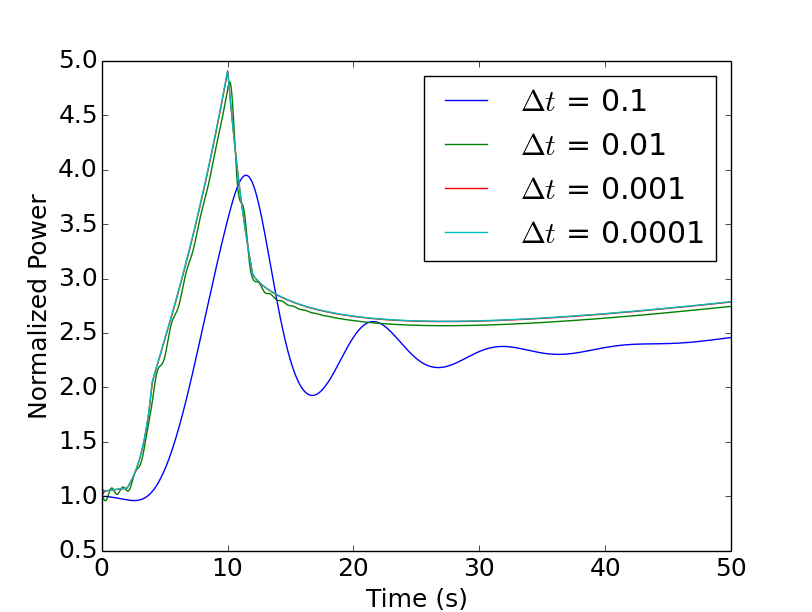
\includegraphics[width=.95\linewidth]{figs/power_case1_conv1.png}
				\caption{Frequency Transform, $\epsilon = 10^{-2}$}
				\label{fig::power_1_1_ft}
			\end{subfigure}%
			\begin{subfigure}{.5\textwidth}
				\centering
				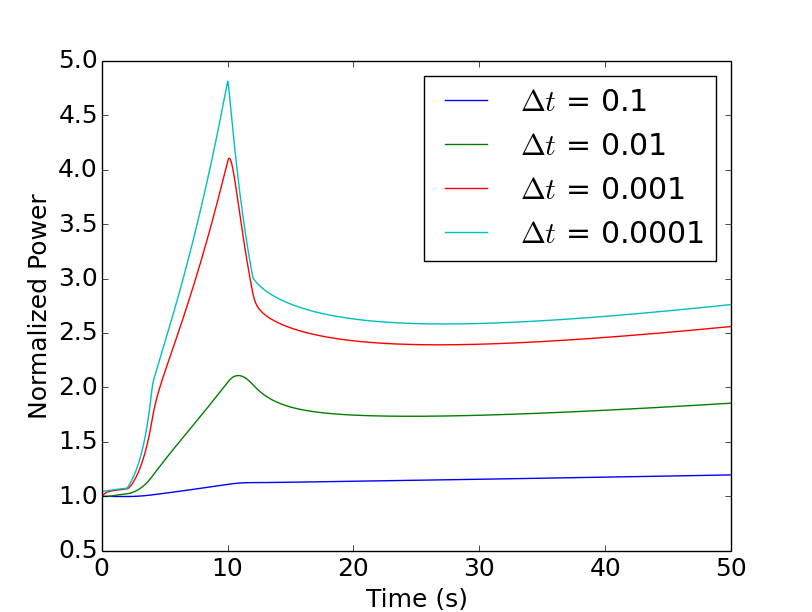
\includegraphics[width=.95\linewidth]{figs/power_case1_conv1_omega0.png}
				\caption{Fully Implicit, $\epsilon = 10^{-2}$}
				\label{fig::power_1_1_fi}
			\end{subfigure}

			\begin{subfigure}{.5\textwidth}
				\centering
				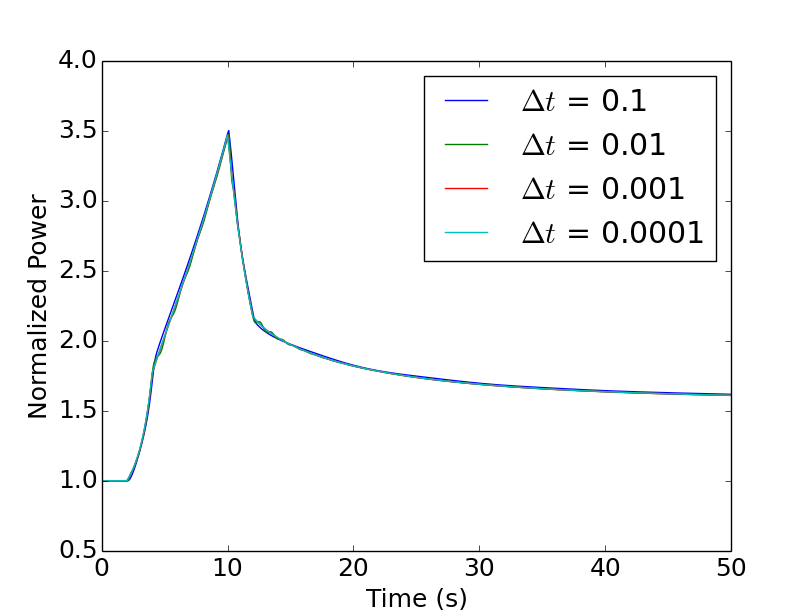
\includegraphics[width=.95\linewidth]{figs/power_case1_conv2.png}
				\caption{Frequency Transform, $\epsilon = 10^{-4}$}
				\label{fig::power_1_2_ft}
			\end{subfigure}%
			\begin{subfigure}{.5\textwidth}
				\centering
				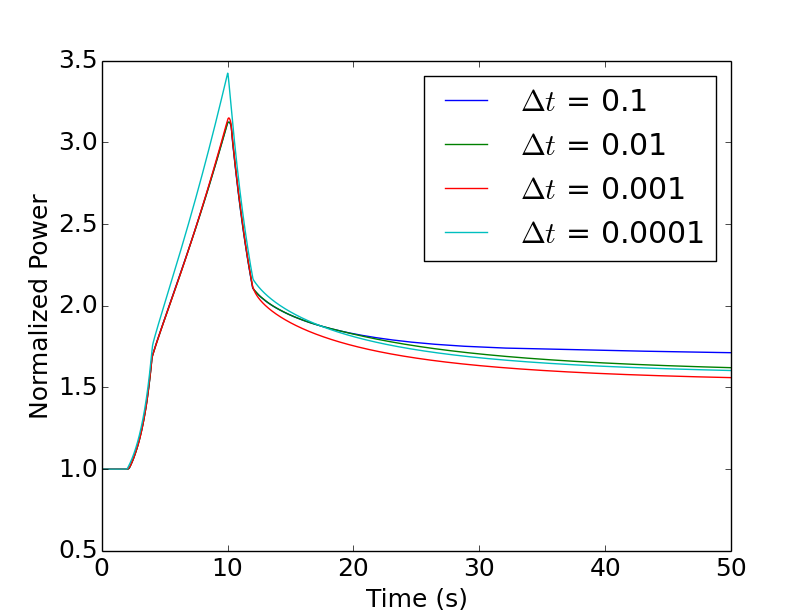
\includegraphics[width=.95\linewidth]{figs/power_case1_conv2_omega0.png}
				\caption{Fully Implicit, $\epsilon = 10^{-4}$}
				\label{fig::power_1_2_fi}
			\end{subfigure}

			\begin{subfigure}{.5\textwidth}
				\centering
				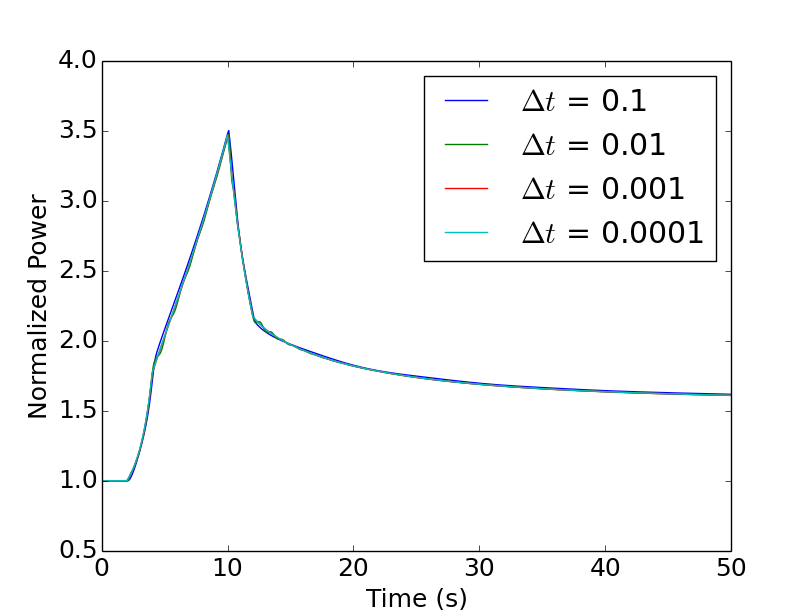
\includegraphics[width=.95\linewidth]{figs/power_case1_conv2.png}
				\caption{Frequency Transform, $\epsilon = 10^{-6}$}
				\label{fig::power_1_3_ft}
			\end{subfigure}%
			\begin{subfigure}{.5\textwidth}
				\centering
				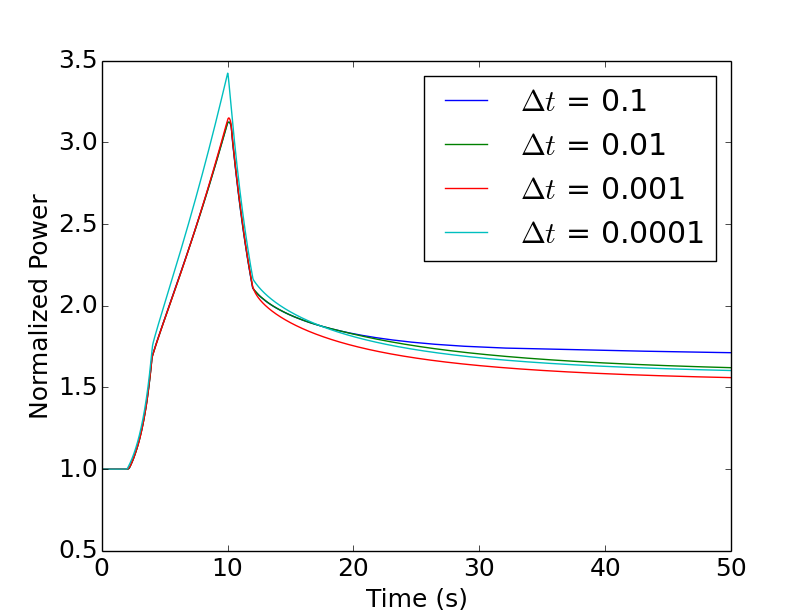
\includegraphics[width=.95\linewidth]{figs/power_case1_conv2_omega0.png}
				\caption{Fully Implicit, $\epsilon = 10^{-6}$}
				\label{fig::power_1_3_fi}
			\end{subfigure}
			\caption{Frequency transform and fully implicit solutions for delayed critical rod withdrawal and insertion with various convergence criteria $\epsilon$ and various time step sizes $\Delta t$.}
			\label{fig::power_1}
		\end{figure}

		\begin{figure}[ht]
			\centering
			\begin{subfigure}{.5\textwidth}
				\centering
				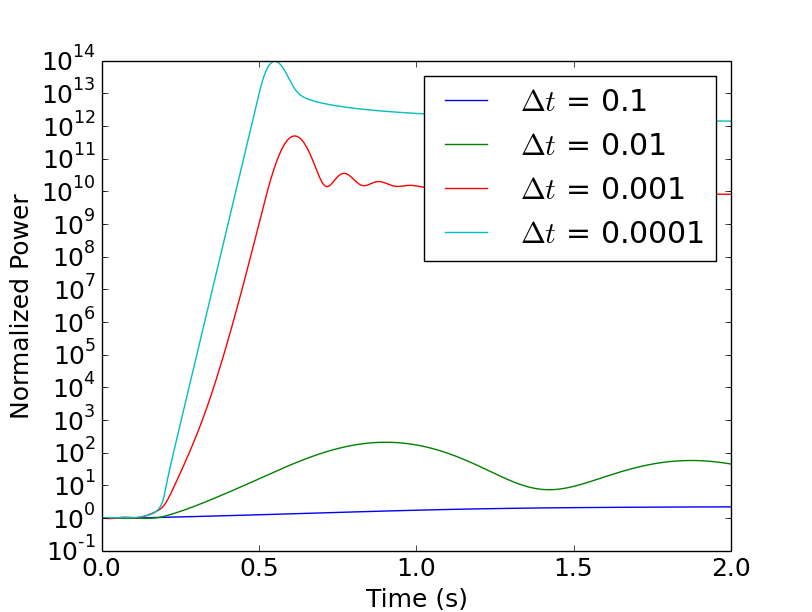
\includegraphics[width=.95\linewidth]{figs/power_case2_conv1.png}
				\caption{Frequency Transform, $\epsilon = 10^{-2}$}
				\label{fig::power_2_1_ft}
			\end{subfigure}%
			\begin{subfigure}{.5\textwidth}
				\centering
				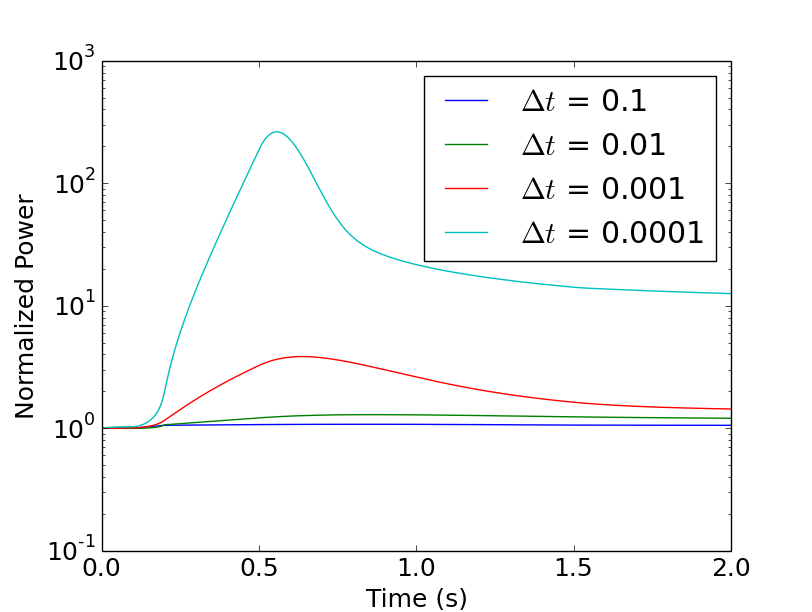
\includegraphics[width=.95\linewidth]{figs/power_case2_conv1_omega0.png}
				\caption{Fully Implicit, $\epsilon = 10^{-2}$}
				\label{fig::power_2_1_fi}
			\end{subfigure}
			
			\begin{subfigure}{.5\textwidth}
				\centering
				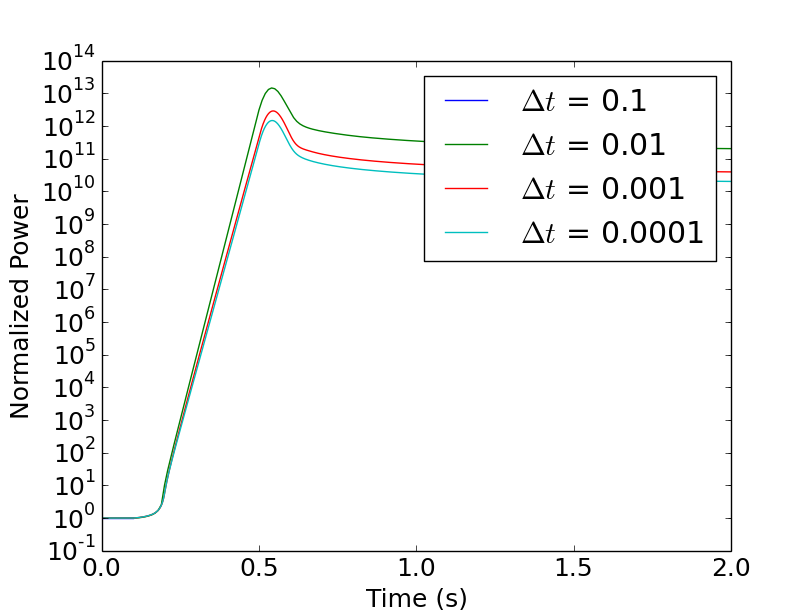
\includegraphics[width=.95\linewidth]{figs/power_case2_conv2.png}
				\caption{Frequency Transform, $\epsilon = 10^{-4}$}
				\label{fig::power_2_2_ft}
			\end{subfigure}%
			\begin{subfigure}{.5\textwidth}
				\centering
				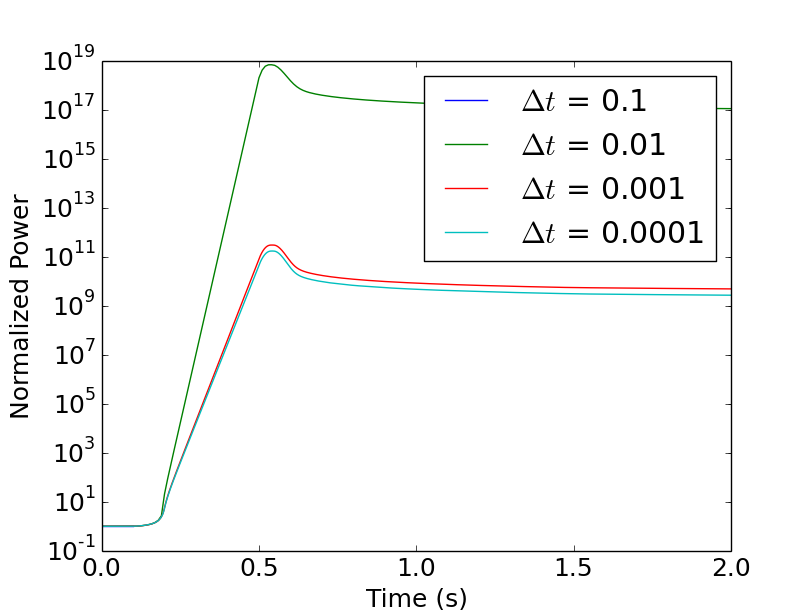
\includegraphics[width=.95\linewidth]{figs/power_case2_conv2_omega0.png}
				\caption{Fully Implicit, $\epsilon = 10^{-4}$}
				\label{fig::power_2_2_fi}
			\end{subfigure}
			
			\begin{subfigure}{.5\textwidth}
				\centering
				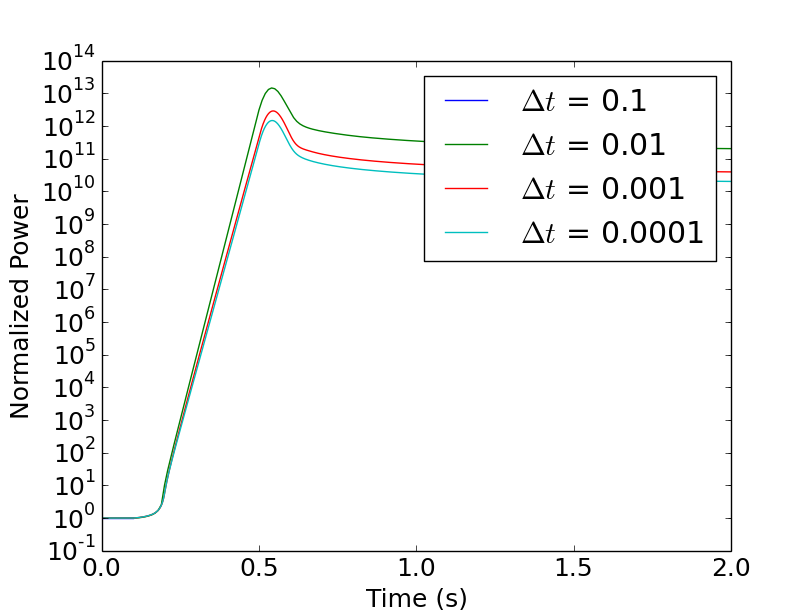
\includegraphics[width=.95\linewidth]{figs/power_case2_conv2.png}
				\caption{Frequency Transform, $\epsilon = 10^{-6}$}
				\label{fig::power_2_3_ft}
			\end{subfigure}%
			\begin{subfigure}{.5\textwidth}
				\centering
				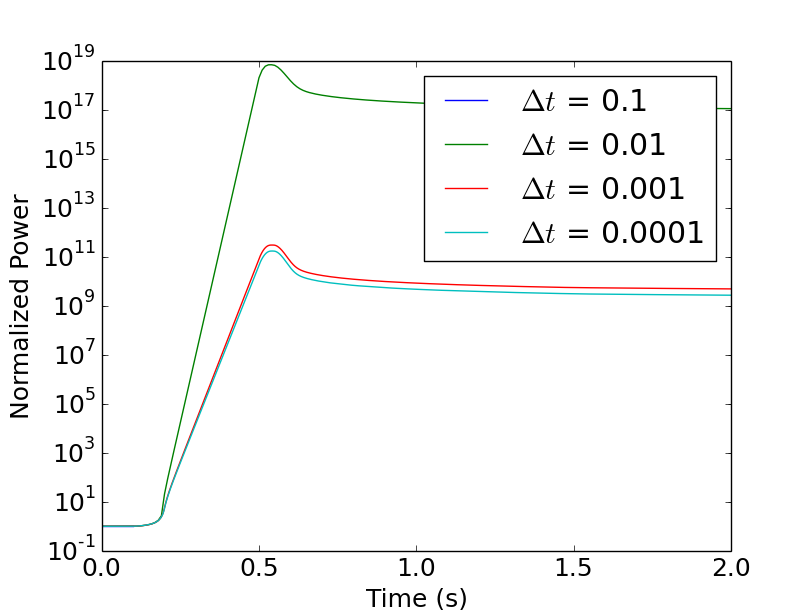
\includegraphics[width=.95\linewidth]{figs/power_case2_conv2_omega0.png}
				\caption{Fully Implicit, $\epsilon = 10^{-6}$}
				\label{fig::power_2_3_fi}
			\end{subfigure}
			\caption{Frequency transform and fully implicit solutions for prompt critical rod withdrawal and scram with various convergence criteria $\epsilon$ and various time step sizes $\Delta t$.}
			\label{fig::power_2}
		\end{figure}

\clearpage
Next we look at the iteration counts as a function of time for both transients. Again, we start with the first transient, the delayed critical bank withdrawal. The results are shown in Fig.~\ref{fig::iter_1}. For loose convergence criteria of $10^{-2}$, both the frequency transform and the fully implicit methods converge in one iteration for all time steps as seen if Fig.~\ref{fig::iter_1_1_ft} and Fig.~\ref{fig::iter_1_1_fi}. When the convergence criteria is tightened, we see interesting results shown in Figs.~\ref{fig::iter_1_2_ft} --~\ref{fig::iter_1_3_fi}. 

Both the frequency transform and fully implicit methods require high iteration counts during control rod movement when the material properties are changing. However, the frequency transform method only requires a few iterations when material properties are constant, such as after the control rod is withdrawn and after the control rod is re-inserted. The fully implicit method still requires a large number of iterations during these periods when the material properties are constant but the flux is still rapidly changing. In fact, the number of iterations seems to follow the magnitude of the change in flux. When the flux is exponentially decreasing after the re-insertion of the rod, the number of iterations required also decreases exponentially. 

The reason the frequency transform is able to solve the transient during these periods of constant material properties but exponential change in flux and power amplitude is the inherent assumption that the flux should change exponentially between time steps that is present in the derivation of the frequency transform.

For the super prompt critical rod ejection transient, similar results are observed. These are shown in Fig.~\ref{fig::iter_2}. Once again, for loose convergence criteria, very few iterations are required for both the frequency transform and the fully implicit methods. During the rod ejection and scram, a very large number of iterations are needed for both methods. However, during periods when the material properties are constant and flux is changing exponentially, the frequency transform method requires very few iterations but the fully implicit method still requires a significant number of iterations.
% iteration counts
		\begin{figure}[ht]
			\centering
			\begin{subfigure}{.5\textwidth}
				\centering
				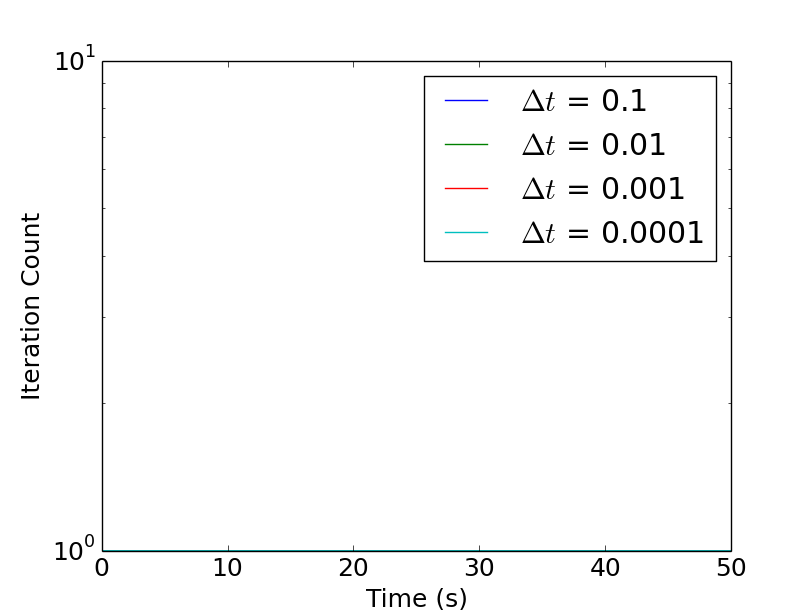
\includegraphics[width=.95\linewidth]{figs/iter_case1_conv1.png}
				\caption{Frequency Transform, $\epsilon = 10^{-2}$}
				\label{fig::iter_1_1_ft}
			\end{subfigure}%
			\begin{subfigure}{.5\textwidth}
				\centering
				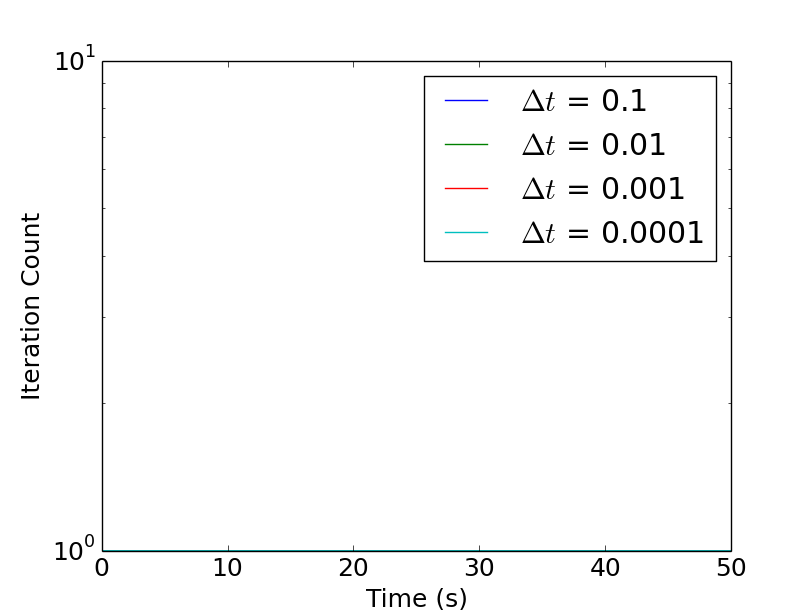
\includegraphics[width=.95\linewidth]{figs/iter_case1_conv1_omega0.png}
				\caption{Fully Implicit, $\epsilon = 10^{-2}$}
				\label{fig::iter_1_1_fi}
			\end{subfigure}
			
			\begin{subfigure}{.5\textwidth}
				\centering
				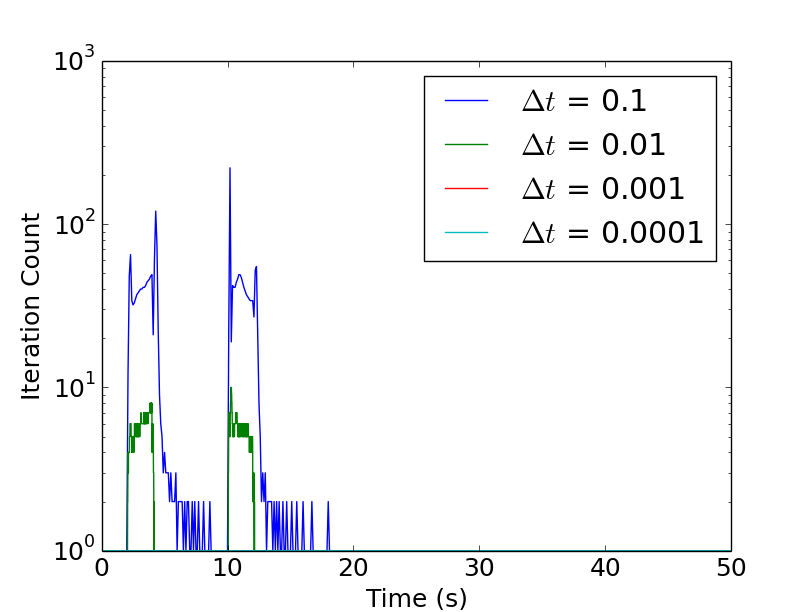
\includegraphics[width=.95\linewidth]{figs/iter_case1_conv2.png}
				\caption{Frequency Transform, $\epsilon = 10^{-4}$}
				\label{fig::iter_1_2_ft}
			\end{subfigure}%
			\begin{subfigure}{.5\textwidth}
				\centering
				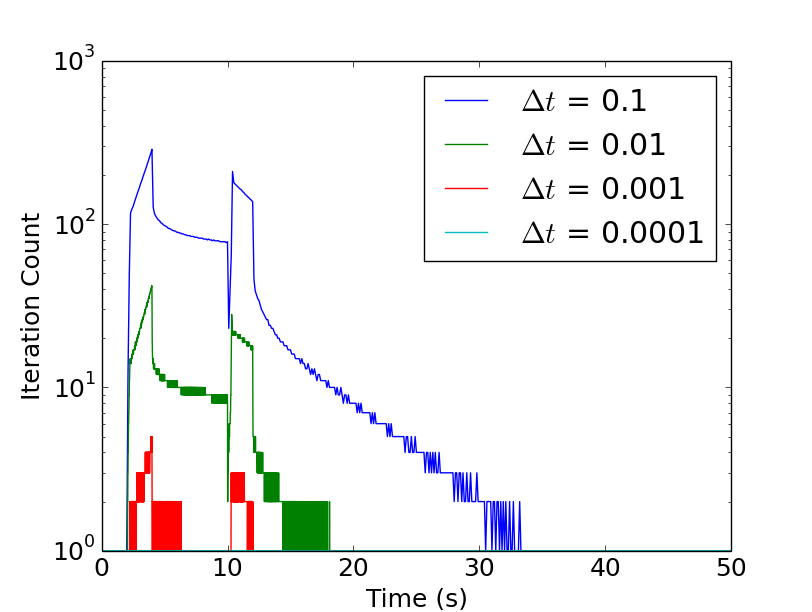
\includegraphics[width=.95\linewidth]{figs/iter_case1_conv2_omega0.png}
				\caption{Fully Implicit, $\epsilon = 10^{-4}$}
				\label{fig::iter_1_2_fi}
			\end{subfigure}
			
			\begin{subfigure}{.5\textwidth}
				\centering
				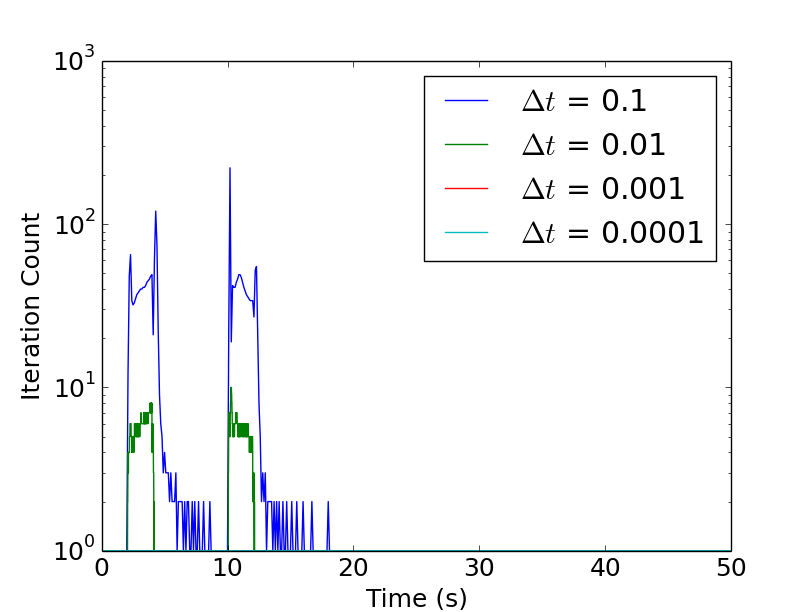
\includegraphics[width=.95\linewidth]{figs/iter_case1_conv2.png}
				\caption{Frequency Transform, $\epsilon = 10^{-6}$}
				\label{fig::iter_1_3_ft}
			\end{subfigure}%
			\begin{subfigure}{.5\textwidth}
				\centering
				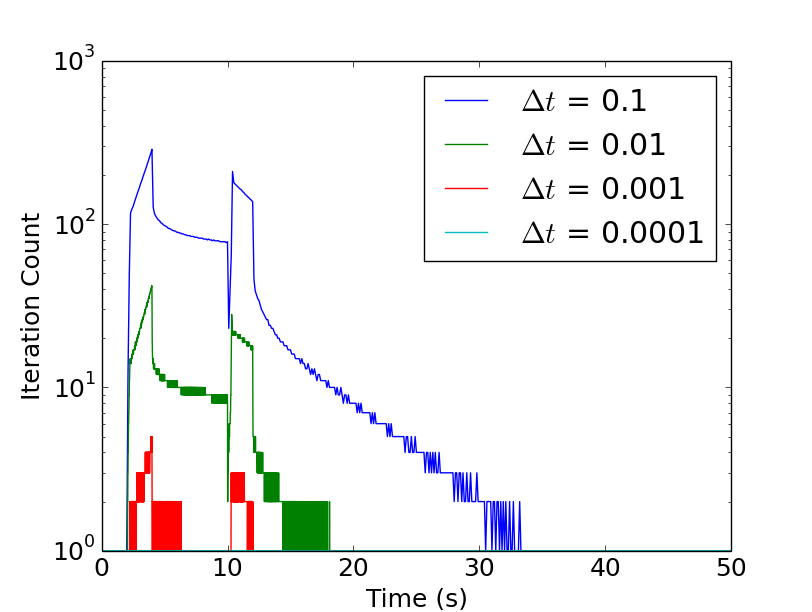
\includegraphics[width=.95\linewidth]{figs/iter_case1_conv2_omega0.png}
				\caption{Fully Implicit, $\epsilon = 10^{-6}$}
				\label{fig::iter_1_3_fi}
			\end{subfigure}
			\caption{Iteration count as a function of time for frequency transform and fully implicit solutions for delayed critical rod withdrawal and insertion with various convergence criteria $\epsilon$ and various time step sizes $\Delta t$.}
			\label{fig::iter_1}
		\end{figure}
		
		\begin{figure}[ht]
			\centering
			\begin{subfigure}{.5\textwidth}
				\centering
				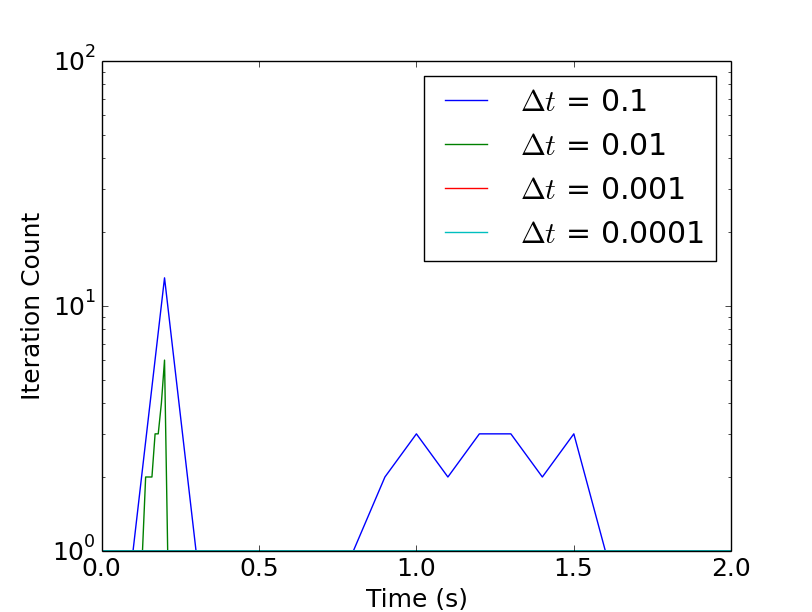
\includegraphics[width=.95\linewidth]{figs/iter_case2_conv1.png}
				\caption{Frequency Transform, $\epsilon = 10^{-2}$}
				\label{fig::iter_2_1_ft}
			\end{subfigure}%
			\begin{subfigure}{.5\textwidth}
				\centering
				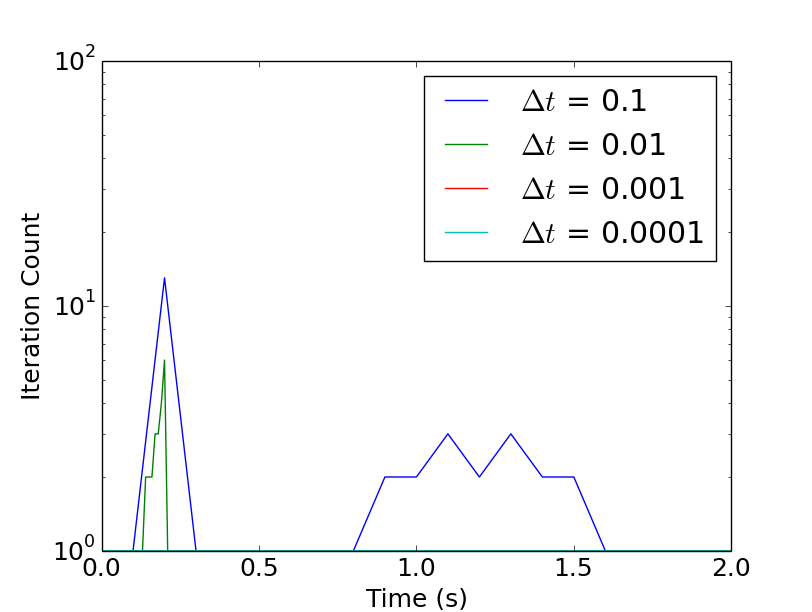
\includegraphics[width=.95\linewidth]{figs/iter_case2_conv1_omega0.png}
				\caption{Fully Implicit, $\epsilon = 10^{-2}$}
				\label{fig::iter_2_1_fi}
			\end{subfigure}
			
			\begin{subfigure}{.5\textwidth}
				\centering
				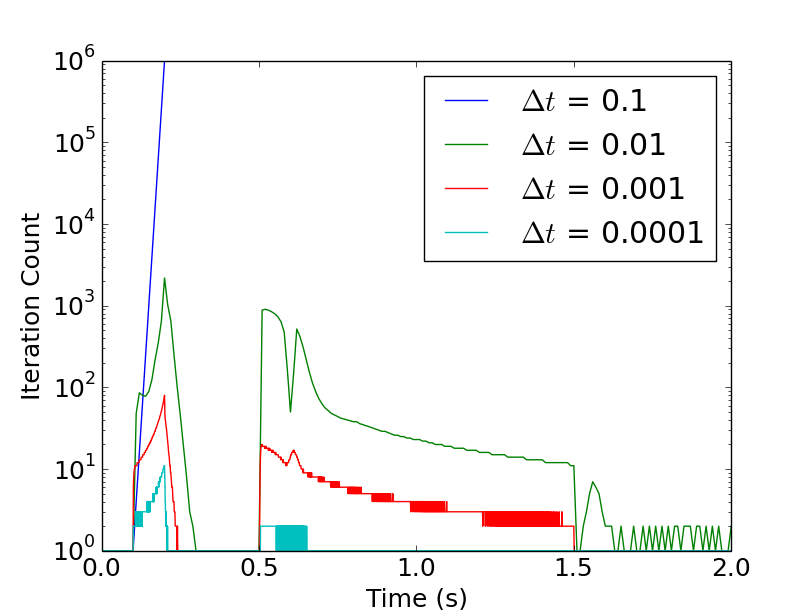
\includegraphics[width=.95\linewidth]{figs/iter_case2_conv2.png}
				\caption{Frequency Transform, $\epsilon = 10^{-4}$}
				\label{fig::iter_2_2_ft}
			\end{subfigure}%
			\begin{subfigure}{.5\textwidth}
				\centering
				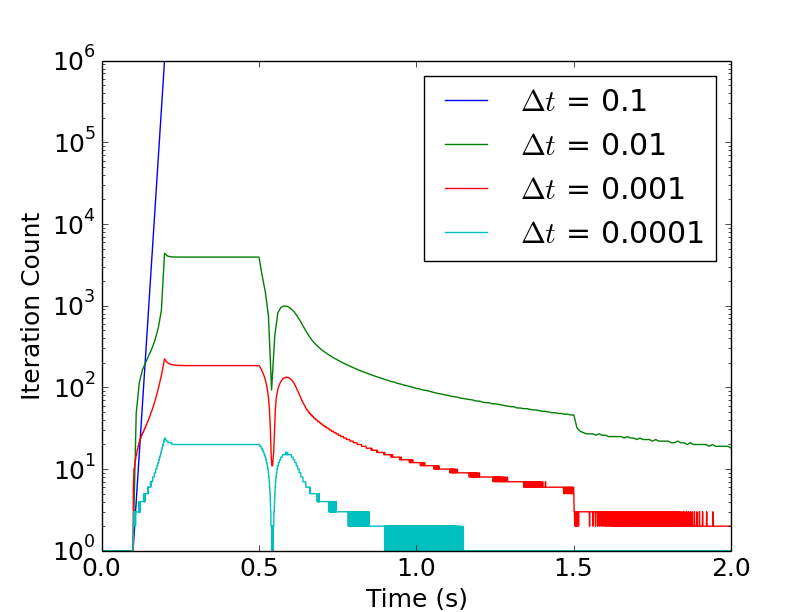
\includegraphics[width=.95\linewidth]{figs/iter_case2_conv2_omega0.png}
				\caption{Fully Implicit, $\epsilon = 10^{-4}$}
				\label{fig::iter_2_2_fi}
			\end{subfigure}
			
			\begin{subfigure}{.5\textwidth}
				\centering
				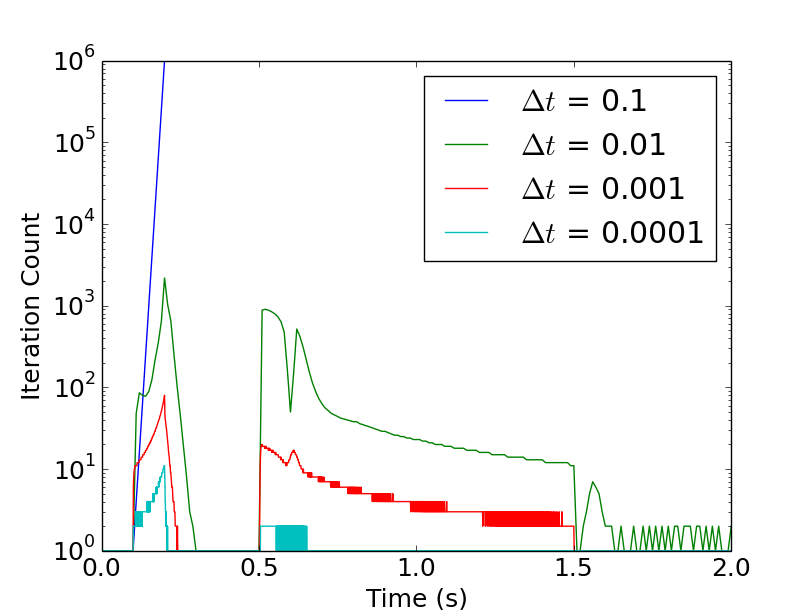
\includegraphics[width=.95\linewidth]{figs/iter_case2_conv2.png}
				\caption{Frequency Transform, $\epsilon = 10^{-6}$}
				\label{fig::iter_2_3_ft}
			\end{subfigure}%
			\begin{subfigure}{.5\textwidth}
				\centering
				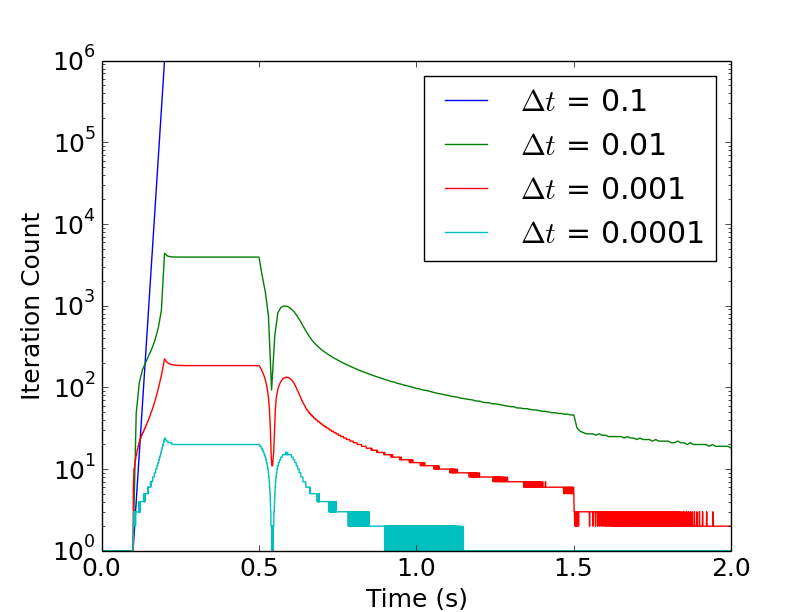
\includegraphics[width=.95\linewidth]{figs/iter_case2_conv2_omega0.png}
				\caption{Fully Implicit, $\epsilon = 10^{-6}$}
				\label{fig::iter_2_3_fi}
			\end{subfigure}
			\caption{Iteration count as a function of time for frequency transform and fully implicit solutions for super prompt critical rod withdrawal and scram with various convergence criteria $\epsilon$ and various time step sizes $\Delta t$.}
			\label{fig::iter_2}
		\end{figure}
	\clearpage
	\paragraph{Part B: Effect of $\omega$ Calculation Schemes}
	In this part, the effect of how $\omega(\vec{r})$ is calculated during each iteration is analyzed. First, the effect of global and local $\omega(\vec{r})$ estimates are compared. The resulting power profiles are plotted for both transients mentioned in \textbf{Part A} in Fig.~\ref{fig::global_local}.
	\begin{figure}[ht]
		\centering
		\begin{subfigure}{.49\textwidth}
			\centering
			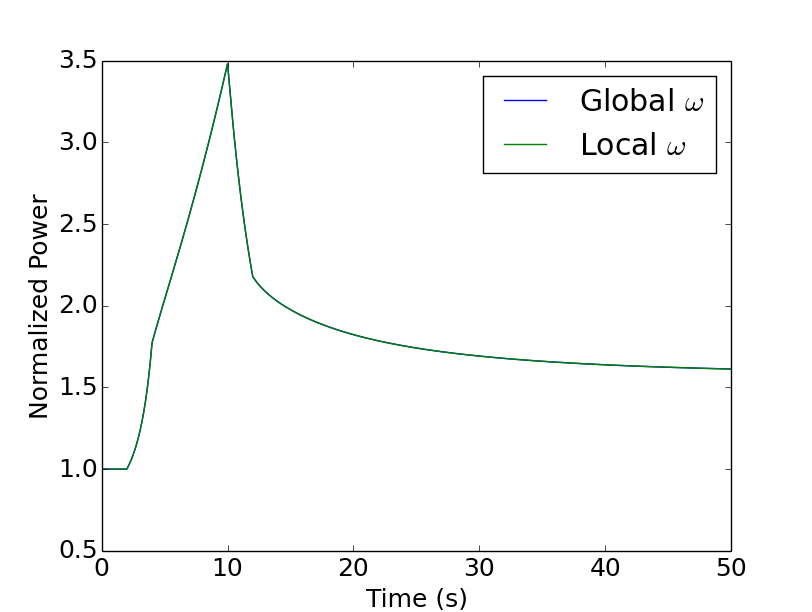
\includegraphics[width=.95\linewidth]{figs/global_local_case1.png}
			\caption{Delayed Critical Bank Withdrawal}
			\label{fig::global_local_case1}
		\end{subfigure}
		\begin{subfigure}{.49\textwidth}
			\centering
			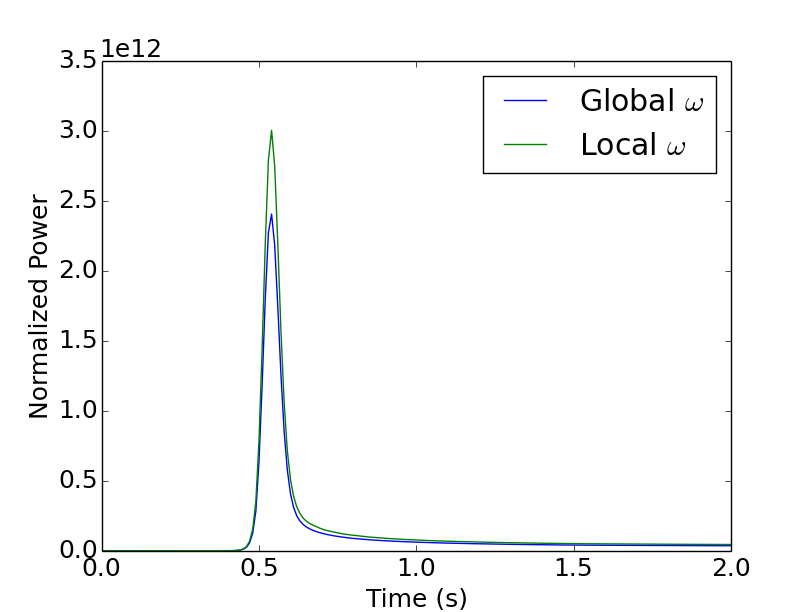
\includegraphics[width=.95\linewidth]{figs/global_local_case2.png}
			\caption{Prompt Critical Rod Ejection}
			\label{fig::global_local_case2}
		\end{subfigure}
		\caption{Frequency transform solutions for both the delayed critical bank withdrawal transient and the super prompt critical rod ejection with scram using both global and local unsynchronized frequencies at a convergence criteria  of $10^{-6}$ and a time step size of $10^{-2}$.}
		\label{fig::global_local}
	\end{figure}
	
	Notice that for the delayed critical bank withdrawal transient, resulting power profiles from using both global and local frequencies align very well. Since the transient is so slow, the estimate of $\omega$ is not as important as the calculated value should be very small. However, for the prompt critical rod ejection in which the flux changes very rapidly, significant deviation between the power profiles is observed. This is likely due to the flux changing rapidly in the center, near the control rod ejection, but far less rapid away from the control rod. 

	Next, for the global frequency case, synchronized and unsynchronized frequency transform calculations are compared. In this implementation, we conduct only a single re-calculation of $\omega$ for the synchronized version. A calculation of the flux is performed using the regular unsynchronized frequency. The appropriate value for $\omega$ is then re-calculated using the calculated flux. Then the flux is re-calculated using the new estimate of $\omega$ and the time step is then progressed. This is of course an approximation since $\omega$ should really be iteratively converged. 
	
	The results are shown in Fig.~\ref{fig::sync}. Again, for the slowly changing delayed critical bank withdrawal transient there is little deviation between the synchronized and unsynchronized. However, for the rapidly changing super prompt critical rod ejection, significant deviation is once again observed between the unsynchronized and synchronized power profiles, especially at the power peak of the transient.
	

	\begin{figure}[ht]
		\centering
		\begin{subfigure}{.49\textwidth}
			\centering
			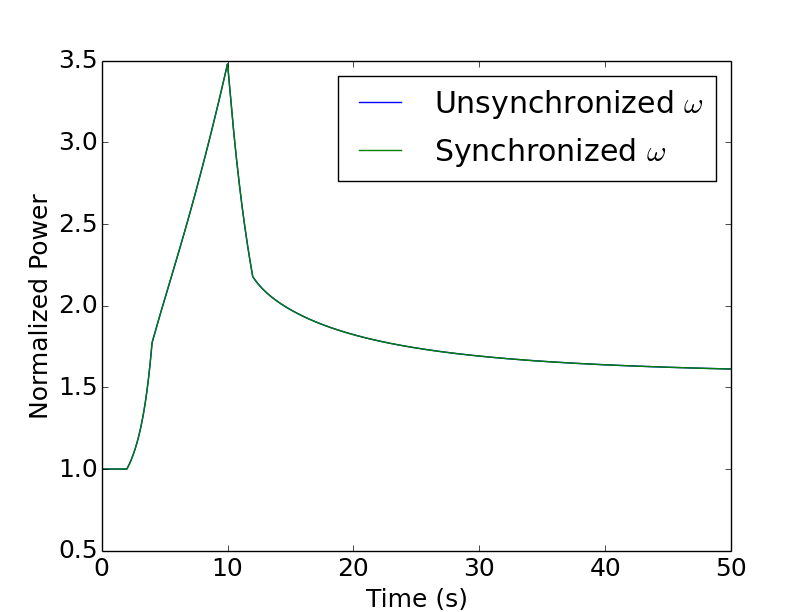
\includegraphics[width=.95\linewidth]{figs/sync_case1.png}
			\caption{Delayed Critical Bank Withdrawal}
			\label{fig::sync_case1}
		\end{subfigure}
		\begin{subfigure}{.49\textwidth}
			\centering
			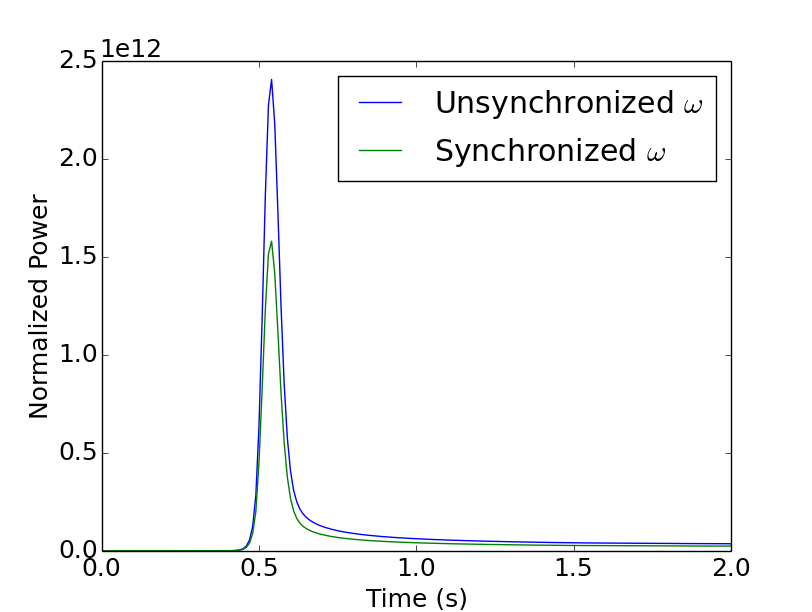
\includegraphics[width=.95\linewidth]{figs/sync_case2.png}
			\caption{Super Prompt Critical Rod Ejection}
			\label{fig::sync_case2}
		\end{subfigure}
		\caption{Frequency transform solutions for both the delayed critical bank withdrawal transient and the super prompt critical rod ejection with scram using both synchronized and unsynchronized global frequencies at a convergence criteria  of $10^{-6}$ and a time step size of $10^{-2}$.}
		\label{fig::sync}
	\end{figure}
\end{document}